\documentclass{article}
% Build mode: arXiv preprint (NeurIPS formatting, author named, no venue notice).
% [final] would print "NeurIPS 2025" in the footer and [preprint] prints "Under
% review"; for an anonymous venue submission, drop the option and anonymise \author.
% neurips.sty loads natbib in author-year mode, which conflicts with the numeric
% bibliography style; building from main.bbl alone (as arXiv does) then fails.
\PassOptionsToPackage{numbers,compress}{natbib}
\usepackage[preprint]{neurips}
\makeatletter
\renewcommand{\@noticestring}{}
\makeatother

\usepackage[utf8]{inputenc}
\usepackage[T1]{fontenc}
\usepackage{hyperref}
\usepackage{url}
\usepackage{booktabs}
\usepackage{amsmath}
\usepackage{graphicx}

\newcommand{\bench}{\texttt{reverie-bench}}

\title{\texttt{reverie-bench}: Repetition Density and the Limits of\\
Outcome Attribution in Agent Memory}

\author{%
  Carlos Inostroza\\
  \texttt{c.inostroza@gmail.com}
}

\begin{document}

\maketitle

\begin{abstract}
Many memory systems for language-model agents learn which memories to retrieve from
task outcomes: after each task, the memories that informed it are credited with its
success or failure. We test this mechanism, outcome attribution, in a complete memory
system on \bench, a benchmark of contextual-bandit tasks in which repetition density
(tasks per distinct context) is controlled and memory is compared with a recency
baseline under the same token cap. In three conditions, including one we predicted
beforehand would favour attribution, attribution changed task success by between
$-0.008$ and $+0.035$, and no difference was significant. We traced where the credit
went: each outcome's credit was spread over about 40 activated nodes, about 70\% of it
went to 34 entity and summary nodes activated on most tasks, and the 600 episodic
memories that hold task-specific precedents received a median of 0.06 outcomes' worth
of evidence each. Retrieval itself improved success over the recency
baseline by $0.041 \pm 0.016$, and a simulated reviewer writing about two lessons per
reviewed session added $0.174 \pm 0.021$ (paired differences averaged over eight
environment instances). Retrieval outperformed recency at 8.3 tasks per context and
underperformed it at 2.0, and scoring whole runs instead of their second halves
reversed the sign of the retrieval effect.
\end{abstract}

\section{Introduction}

Memory systems for language-model agents store records of past tasks and retrieve the
relevant ones when a similar task arrives~\cite{expel,memp,synapse}. A common extension
uses task outcomes to decide which stored memories are worth retrieving. The system
records which memories each retrieval returned, observes whether the task that followed
succeeded, and updates a usefulness estimate for each of those
memories~\cite{whentoforget,romerl}. Work that trains memory-management policies with
reinforcement learning faces the same credit-assignment problem and addresses it with
denser or more targeted reward~\cite{memt,treecredit,memoryr2,himpo,metacog,attrimem}.

We built a memory system with outcome attribution, which we call Reverie, and found
that attribution did not improve task success. This paper reports that result, a
measurement of how the system distributed credit, and the benchmark on which we
measured both. We designed the benchmark so that the contribution of memory can be
separated from properties of the workload. Four choices in its design affect the
results we report:
\begin{enumerate}
\item Memory is compared with a recency baseline that receives the most recent task
  records under the same token cap. Our agent cannot learn across tasks without memory,
  so a comparison with no memory at all would favour any memory system.
\item Repetition density, the number of tasks per distinct context, is a controlled
  variable.
\item Results are averaged over several randomly generated environment instances.
\item The part of each run that is scored is fixed in advance, because a memory system
  starts each run empty.
\end{enumerate}

Our contributions are:
\begin{itemize}
\item \bench, a benchmark with these properties (\S\ref{sec:bench}). Using it, we find
  that retrieval outperforms the recency baseline at 8.3 tasks per context and
  underperforms it at 2.0 (\S\ref{sec:density}), and that scoring whole runs instead of
  their second halves reverses the sign of that comparison (\S\ref{sec:protocol}).
\item A null result for outcome attribution in three conditions, with the size of
  effect the data can exclude, and a measurement showing that most of the credit goes
  to nodes activated on most tasks rather than to the memories retrieval depends on
  (\S\ref{sec:attribution}).
\item An evaluation of a review channel in which a simulated reviewer writes lessons
  into memory, varying the reviewer's frequency, accuracy, error type and scope, with a
  check of the channel's main mechanism on a language model (\S\ref{sec:review}).
\item A negative result for a scope-validation guard we designed, tested against four
  predictions made before the experiment (\S\ref{sec:guard}).
\end{itemize}

\section{\texttt{reverie-bench}}
\label{sec:bench}

\paragraph{Tasks.}
Each task family in \bench\ is a contextual bandit. A task presents a set of feature
values and a set of strategies, and a hidden rule table assigns each context a correct
strategy. Choosing it succeeds except with a flake probability of 0.05; any other
choice fails. Feature values are drawn afresh for every task, so an agent can improve
only by learning the mapping from features to strategies.

The main family, used for all results in this paper, models on-call incident response.
A task has three features: the affected service (12 values), the symptom (6 values) and
the severity (3 values). The six strategies are restart, rollback, scale out, clear
cache, fail over and page the owner. Severity has no effect on the correct strategy. For
two of the six symptoms the correct strategy is the same on every service, and for the
other four it depends on the service, so there are 72 relevant contexts. A uniformly
random choice succeeds with probability $\frac{1}{6} \times 0.95 = 0.158$. The rule
table is generated from a seed, and we call each generated table an \emph{environment
instance}. In the drift condition, the correct strategy changes at task 300 for a fixed
half of the service--symptom pairs. The benchmark also includes three smaller families
with six to eight contexts, which we do not use here.

\paragraph{Repetition density.}
We define repetition density as the number of tasks in a run divided by the number of
relevant contexts. Runs have 600 tasks, which gives 8.3 tasks per context for the
family above. To vary density we change the size of the family at a fixed task budget:
30 services and 10 symptoms give 2.0 tasks per context, and 60 services and 20 symptoms
give 0.5.

\paragraph{Agent.}
All conditions use the same scripted policy, so they differ only in the evidence the
policy receives. An evidence item consists of a context, a strategy, an outcome and a
weight. With probability 0.12 the agent chooses a strategy at random. Otherwise each
item adds $w s^2$ to its strategy's score if it records a success and subtracts
$w s^2$ if it records a failure, where $w$ is the item's weight and $s$ is the fraction
of feature values its context shares with the task. The agent chooses the
highest-scoring strategy, or a random one if the total weight of the evidence is below
0.15. The policy keeps no state between tasks, so any improvement over a run comes from
the evidence it is given.

\paragraph{Conditions.}
In the \emph{no-memory} condition the agent receives no evidence. In the \emph{replay}
condition it receives the most recent task records, newest first, up to a cap of 1,200
tokens; these prompts average 1,146 tokens. In the \emph{Reverie} condition it receives
the brief returned by the memory system described in \S\ref{sec:system}, under the same
cap; these briefs average 794 tokens and about nine items. The \emph{review} condition
adds a simulated reviewer to Reverie.

\paragraph{Simulated reviewer.}
A run is divided into sessions of 20 tasks. At the end of each session the reviewer is
consulted with probability $f$, the review frequency. When consulted, it picks up to
two failed tasks from the session and writes a lesson for each, consisting of a context
and a strategy. The reviewer has access to the true rule table. With probability $a$,
its accuracy, a lesson names the correct strategy; otherwise it names a wrong strategy
according to one of three error types. Under \emph{random} errors each lesson is wrong
independently, with the wrong strategy drawn uniformly. Under \emph{per-context} errors
a fixed fraction $1-a$ of contexts always receive the same wrong strategy. Under
\emph{fixed-answer} errors each lesson is wrong independently, and every wrong lesson
names the first incorrect strategy in a fixed list. By default a lesson's context names
the service and the symptom, which is the correct scope for the rule. In the
\emph{over-broad} condition it names only the service, so one lesson claims to cover all
six symptoms of that service. Lessons are stored as procedural memories and, when
retrieved, enter the agent's vote as successes with weight 3. Since the reviewer knows
the true rule table, the review results describe a well-informed reviewer; the accuracy
and error-type conditions measure how the benefit changes when that reviewer is wrong.

\paragraph{Protocol and statistics.}
The primary measure is the success rate over tasks 301--600. It excludes the part of
the run in which memory is being filled; \S\ref{sec:protocol} reports how the results
change when the whole run is scored. A seed fixes the task sequence and the agent's
random choices, and all conditions run with a given seed face the same tasks in the same
order. Except in \S\ref{sec:protocol}, all results come from one environment instance,
with 6 to 16 seeds per condition as stated. Outcomes within a run are correlated,
because a rule learned early helps for the rest of the run, so we treat the run as the
unit of analysis. Reported intervals are $\pm 2$ standard errors across runs, and
differences between conditions are paired by seed. For results averaged over
environment instances, the unit is the instance.

The environment is deterministic given its seeds.\footnote{An earlier version of the
benchmark derived the rule table from Python's built-in \texttt{hash}, which is salted
per process, so the same seed produced a different environment in each interpreter: one
configuration gave success rates of 0.368, 0.400 and 0.408 in three processes. The rule
table is now derived from a BLAKE2b hash.} The memory system is not, because its
recency score uses wall-clock time and its node identifiers contain random bits.
Repeating one seed four times gave second-half success rates with a standard deviation
of 0.041, compared with about 0.05 across seeds. This variation is included in our
intervals.

\section{Memory system}
\label{sec:system}

Reverie stores memory as a graph in SQLite. After each task it writes an episode node
recording the context, the chosen strategy and the outcome, linked to one entity node
for each feature value and strategy name. Every 10 tasks a consolidation pass writes
failure-mode summaries, groups related nodes into communities with a summary node for
each, and runs the scope guard described below. Reviewer lessons are written directly
as procedural nodes linked to the entities they name.

\paragraph{Retrieval.}
The query for a task is its context. Candidate nodes are found by full-text search, by
vector search and by exact matching of the query's feature values to entity nodes; the
three rankings are combined by reciprocal rank fusion, with the exact matches weighted
double. The association channel spreads activation up to three hops from the top
candidates and scores each node by its activation, recency and estimated utility, among
other factors. The
precision channel admits nodes that match the query directly: those linked to at least
95\% of the query's entities, weighted by inverse document frequency, and those whose
own entities are at least 95\% contained in the query, which admits lessons that omit a
feature. Admitted nodes are ranked by the product of coverage, containment and
estimated utility, and they may use up to half of the token budget. The two channels
are merged into a brief under the 1,200-token cap.

\paragraph{Outcome attribution.}
Each retrieval is logged with the activation of every node it reached. When the task's
outcome is recorded, one unit of credit is divided among those nodes in proportion to
their activation, normalised within each channel, and added to each node's Beta
posterior: to $\alpha$ on success and to $\beta$ on failure, starting from
$\mathrm{Beta}(1,1)$. A node's estimated utility is the 25th percentile of its
posterior, which is 0.25 before the node has received any credit. Utility multiplies the
ranking score in both retrieval channels. In one variant the agent also weights the vote
of each retrieved episode by $\max(0.1, 2u)$, where $u$ is the episode's utility;
lessons are not weighted.

\paragraph{Scope guard.}
At each consolidation, the guard examines every reviewer lesson that has at least eight
episodes inside its claimed scope, meaning episodes linked to all of the entities the
lesson names. If fewer than 60\% of those episodes succeeded, it looks for an entity
outside the lesson's scope that splits them into a group with a success rate of at least
60\% and an information gain of at least 0.05. If it finds one, the lesson is replaced by
a copy whose scope includes that entity; if not, the lesson is marked as contested. The
guard uses only episode outcomes and never reads the strategy a lesson recommends.

\section{Results}

\subsection{Retrieval and repetition density}
\label{sec:density}

\begin{figure}[t]
\centering
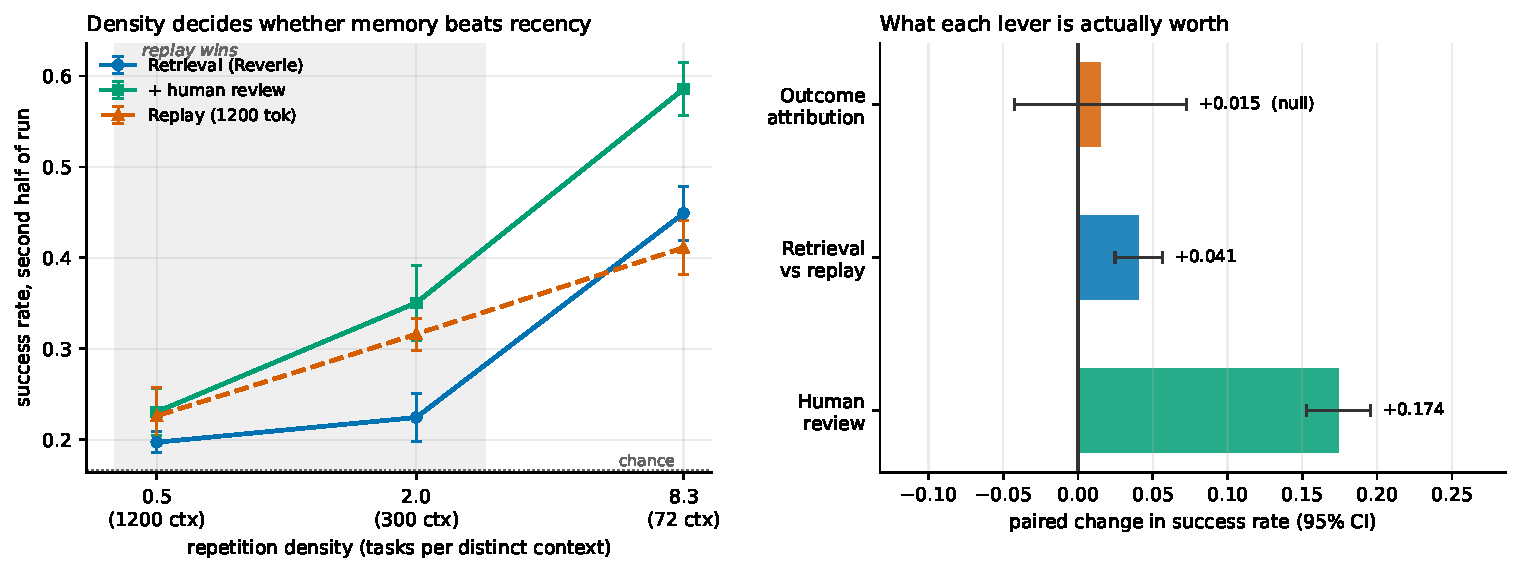
\includegraphics[width=\textwidth]{figures/fig1.pdf}
\caption{(a) Success over tasks 301--600 against repetition density, varied by the
number of contexts at a fixed budget of 600 tasks (6 seeds per point). (b) Paired
differences in the same measure with 95\% intervals. The attribution bars compare
attribution used for ranking and vote weighting against attribution disabled, on one
environment instance with 8 seeds (\S\ref{sec:attribution}). The retrieval and review
bars are averages over eight environment instances with 6 seeds each
(\S\ref{sec:protocol}).}
\label{fig:one}
\end{figure}

\begin{table}[t]
\centering
\caption{Success over tasks 301--600 against repetition density. The number of
contexts grows at a fixed budget of 600 tasks. Six seeds per cell. The last column is
the paired difference between Reverie and replay.}
\label{tab:density}
\small
\begin{tabular}{rrcccc}
\toprule
Contexts & Tasks/context & Reverie & Reverie + review & Replay & Reverie $-$ replay \\
\midrule
72 & 8.3 & $0.449 \pm 0.030$ & $0.586 \pm 0.029$ & $0.411 \pm 0.029$ & $+0.038 \pm 0.014$ \\
300 & 2.0 & $0.224 \pm 0.026$ & $0.351 \pm 0.041$ & $0.316 \pm 0.018$ & $-0.092 \pm 0.020$ \\
1{,}200 & 0.5 & $0.197 \pm 0.012$ & $0.231 \pm 0.026$ & $0.226 \pm 0.031$ & $-0.029 \pm 0.027$ \\
\bottomrule
\end{tabular}
\end{table}

At 8.3 tasks per context, Reverie's success exceeded replay's by $0.038 \pm 0.014$
(Table~\ref{tab:density}, Figure~\ref{fig:one}a). At 2.0 tasks per context replay was
ahead by $0.092 \pm 0.020$, and at 0.5 by $0.029 \pm 0.027$, with both conditions close
to the chance rate of 0.158. Retrieval has an advantage over recency when a precedent
for the current context exists in memory but is not among the most recent records. At
low density the first condition often fails, because the context may not have occurred
before. In the three smaller families of \bench\ the second fails, because a 1,200-token
window typically holds several records for every context.

Review raised Reverie's success by $0.137 \pm 0.024$ at 8.3 tasks per context and by
$0.126 \pm 0.036$ at 2.0. At 0.5 tasks per context its effect, $0.033 \pm 0.033$, was not
significant. With at most two lessons per reviewed session and 1,200 contexts, most
contexts receive no lesson in a 600-task run.

\subsection{Scoring window and environment instance}
\label{sec:protocol}

\begin{table}[t]
\centering
\caption{Paired effects under two scoring windows. Left: the environment instance used
in the rest of the paper, 16 seeds. Right: eight environment instances with 6 seeds
each; the interval treats the instance as the unit ($n = 8$).}
\label{tab:protocol}
\small
\begin{tabular}{llcc}
\toprule
Effect & Scored tasks & One instance & Eight instances \\
\midrule
Reverie $-$ replay & 301--600 & $+0.026 \pm 0.027$ & $+0.041 \pm 0.016$ \\
                   & 1--600   & $-0.044 \pm 0.021$ & $-0.026 \pm 0.015$ \\
\addlinespace
Review $-$ Reverie & 301--600 & $+0.185 \pm 0.033$ & $+0.174 \pm 0.021$ \\
                   & 1--600   & $+0.146 \pm 0.021$ & $+0.135 \pm 0.020$ \\
\bottomrule
\end{tabular}
\end{table}

Table~\ref{tab:protocol} reports the retrieval and review effects under two scoring
windows, on the single environment instance used elsewhere in the paper and averaged
over eight instances. Scoring the whole run reversed the sign of the retrieval effect
in both designs. Over tasks 1--600, Reverie was below replay by $0.044 \pm 0.021$ on the
single instance and by $0.026 \pm 0.015$ across instances, and it was below replay on all
eight instances. Reverie begins each run with an empty graph, while replay is
informative from the second task, so whole-run scores include a period in which memory
is still being filled. Which window is appropriate depends on the deployment being
modelled: a long-running deployment spends most of its time in the regime the second
half measures, and one that is restarted often is closer to the whole run. The review
effect was positive under both windows.

The environment instance also mattered. Across the eight instances, the second-half
retrieval effect ranged from $-0.007$ to $+0.061$ and was positive in seven. On the
single instance, the interval included zero even with 16 seeds. Seeds vary the order of
tasks but not the rule table, so intervals computed over seeds from one instance do not
reflect variation between instances. Results for each instance are in
Appendix~\ref{app:instances}.

\subsection{Outcome attribution}
\label{sec:attribution}

We compared three arms: attribution disabled, in which every posterior stays at its
prior and utility has no effect; attribution used for retrieval ranking; and attribution
used for ranking and for weighting episode votes. We ran them in three conditions: the
static environment, the drift condition, and a fallible-lesson condition in which a
reviewer with accuracy 0.6 was consulted after half of the sessions. Before running the
last condition we predicted that attribution would help there. Lessons are few and are
retrieved often, so each should accumulate evidence quickly, and 40\% of them are wrong,
so there is something for attribution to correct.

\begin{table}[t]
\centering
\caption{Success over tasks 301--600 with outcome attribution disabled, used for
retrieval ranking, and used for ranking and episode vote weighting, and paired
differences from the disabled arm. One environment instance, 8 seeds. Intervals on the
success rates range from $\pm 0.012$ to $\pm 0.047$.}
\label{tab:attribution}
\small
\begin{tabular}{lccccc}
\toprule
& \multicolumn{3}{c}{Success} & \multicolumn{2}{c}{Difference from disabled} \\
\cmidrule(lr){2-4}\cmidrule(lr){5-6}
Condition & Disabled & Ranking & Ranking + votes & Ranking & Ranking + votes \\
\midrule
Static & 0.433 & 0.438 & 0.460 & $+0.005 \pm 0.017$ & $+0.027 \pm 0.034$ \\
Drift & 0.351 & 0.386 & 0.377 & $+0.035 \pm 0.035$ & $+0.026 \pm 0.035$ \\
Fallible lessons & 0.532 & 0.526 & 0.525 & $-0.007 \pm 0.073$ & $-0.008 \pm 0.058$ \\
\bottomrule
\end{tabular}
\end{table}

No arm differed significantly from the disabled arm in any condition
(Table~\ref{tab:attribution}). The point estimates range from $-0.008$ to $+0.035$, and
the largest upper bound is $+0.070$. The data therefore cannot exclude an effect as large
as that of retrieval ($+0.041$), but they exclude one as large as that of review.

\begin{table}[t]
\centering
\caption{Where attribution credit went: nodes of each type at the end of a 600-task
run, their share of all credit, and the median credit per node in units of one outcome.
Fallible-lesson condition with attribution used for ranking and votes; means over four
runs.}
\label{tab:credit}
\small
\begin{tabular}{lrrr}
\toprule
Node type & Nodes & Share of credit & Median credit per node \\
\midrule
Entity (names a feature value or strategy) & 27 & 47\% & 7.70 \\
Failure-mode summary & 7 & 24\% & 20.52 \\
Episode & 600 & 18\% & 0.06 \\
Lesson & 49 & 9\% & 0.36 \\
Community summary & 18 & 2\% & 0.23 \\
\bottomrule
\end{tabular}
\end{table}

To find out why, we measured where the credit went in four runs of the fallible-lesson
condition with attribution fully enabled (Table~\ref{tab:credit}). Credit is conserved:
each attributed outcome (590 of the 600 in a run) distributes one unit, divided among
the nodes its retrieval activated, 40 on average. About 70\% of the credit went to 34
nodes that retrieval activates on most tasks: 27 entity nodes, each of which only names a
feature value or a strategy, and 7 failure-mode summaries. The entity nodes are matched
exactly to the query's feature values and then seed the spreading activation, so they
are among the most activated nodes in every retrieval that involves their value. The
600 episodes, which
contain the task-specific precedents that retrieval depends on, received 18\% between
them, a median of 0.06 units each, and lessons received a median of 0.36 units. A
$\mathrm{Beta}(1,1)$ posterior that receives a fraction of one observation barely moves.
At the end of a run, 32\% of nodes had received no credit at all, and the median utility
was 0.250, the prior value.

As a result, evidence accumulates mainly on nodes that are activated whatever the task,
where it says least about any one memory. A node activated on most tasks is credited with
most outcomes regardless of its contribution, so its posterior tracks the overall success
rate. RoMeRL describes this as misleading updates to co-retrieved
memories~\cite{romerl}, and Simsek~\cite{whentoforget} notes that outcome co-occurrence
statistics of this kind are associational. Excluding entity and summary
nodes from credit would not be enough on its own: if their share were redistributed to
episodes and lessons in proportion to what those already receive, the median episode
would reach about 0.2 units in a 600-task run. One further detail limits our test of the
prediction for the fallible-lesson condition. Vote weighting applies to episodes and not
to lessons, so attribution could act on a wrong lesson only by lowering its rank.

\subsection{Review channel}
\label{sec:review}

\begin{table}[t]
\centering
\caption{Success over tasks 301--600 with review. Left: review frequency, with accurate
lessons (8 seeds). Right: reviewer accuracy with random errors, at review frequency 0.5
(6 seeds). Differences are paired against no review.}
\label{tab:review}
\small
\begin{tabular}{lcc@{\hskip 2em}lcc}
\toprule
Frequency & Success & Difference & Accuracy & Success & Difference \\
\midrule
None & 0.450 &                   & None & 0.446 & \\
0.05 & 0.482 & $+0.032 \pm 0.036$ & 0.4 & 0.495 & $+0.049 \pm 0.030$ \\
0.10 & 0.487 & $+0.037 \pm 0.042$ & 0.6 & 0.513 & $+0.067 \pm 0.047$ \\
0.25 & 0.502 & $+0.051 \pm 0.041$ & 0.8 & 0.592 & $+0.147 \pm 0.035$ \\
0.50 & 0.614 & $+0.163 \pm 0.047$ & 1.0 & 0.610 & $+0.164 \pm 0.022$ \\
1.00 & 0.668 & $+0.217 \pm 0.034$ &     &       & \\
\bottomrule
\end{tabular}
\end{table}

Lessons from the simulated reviewer raised success substantially
(Table~\ref{tab:review}). With accurate lessons, success rose with review frequency, from
0.450 without review to 0.614 when half the sessions were reviewed and 0.668 when all
were, a paired increase of $0.217 \pm 0.034$. The increase had not levelled off at full
review. Even then the reviewer writes at most 60 lessons in a run, fewer than the 72
contexts, so coverage is still growing when the run ends. At review frequency 0.5,
success rose with reviewer accuracy. At accuracy 0.4, when most lessons are wrong, it was
still above the no-review baseline, by $0.049 \pm 0.030$.

\begin{table}[t]
\centering
\caption{Paired change in success over tasks 301--600 relative to no review under the
same conditions, at review frequency 0.5. Error types: 8 seeds, no-review baseline
0.440. Scope: accuracy 1.0, 16 seeds, baseline 0.451. Drift: accuracy 1.0, 8 seeds,
baseline 0.369.}
\label{tab:reviewer}
\small
\begin{tabular}{lcc}
\toprule
Reviewer & Accuracy 0.8 & Accuracy 0.5 \\
\midrule
Random errors & $+0.115 \pm 0.024$ & $+0.071 \pm 0.043$ \\
Per-context errors & $+0.124 \pm 0.050$ & $+0.034 \pm 0.036$ \\
Fixed-answer errors & $+0.122 \pm 0.045$ & $+0.047 \pm 0.038$ \\
\midrule
& \multicolumn{2}{c}{Accuracy 1.0} \\
\cmidrule(lr){2-3}
Correct scope (service and symptom) & \multicolumn{2}{c}{$+0.164 \pm 0.021$} \\
Over-broad scope (service only) & \multicolumn{2}{c}{$-0.016 \pm 0.015$} \\
\addlinespace
Drift at task 300, reviewer throughout & \multicolumn{2}{c}{$+0.107 \pm 0.031$} \\
Drift at task 300, reviewer stops at drift & \multicolumn{2}{c}{$+0.063 \pm 0.022$} \\
\bottomrule
\end{tabular}
\end{table}

Wrong lessons reduced the benefit of review, but under none of the three error types
did they reduce success below the no-review baseline (Table~\ref{tab:reviewer}). With
half of all lessons wrong, the estimates ranged from $+0.034 \pm 0.036$ for per-context
errors, the only one not significantly above the baseline, to $+0.071 \pm 0.043$ for
random errors. We had expected consistent errors to do more damage than random ones,
because a repeated mistake is not averaged out. Per-context errors did have the lowest
estimate at accuracy 0.5, but the differences between error types were within the
intervals. We attribute the limited damage to the episodes: a wrong lesson for a context
is retrieved together with episodes from the same context in which its strategy failed,
and the agent's vote counts both.

A lesson stated at too broad a scope was the only reviewer condition with a negative
estimate. When the reviewer named only the service, success was $0.016 \pm 0.015$ below
the no-review baseline; when the same reviewer named both the service and the symptom,
success was $0.164 \pm 0.021$ above it. An over-broad lesson applies to the symptoms for
which its strategy is wrong, including contexts in which no episode yet exists to
contradict it.

Lessons written before the environment changed remained useful after the change. In
the drift condition, a reviewer consulted throughout the run raised success by
$0.107 \pm 0.031$, and a reviewer who stopped at the drift point raised it by
$0.063 \pm 0.022$. Half of the service--symptom pairs keep their correct strategy after
the drift, so about half of the earlier lessons remain correct.

\paragraph{Check on a language model.}
The argument above assumes that the agent weighs a lesson against contradicting
episodes. Our scripted policy does so by construction, so we tested whether a language
model does the same. We gave \texttt{claude-opus-5} a prompt that described an incident,
listed the six strategies and included a memory brief. The brief contained one lesson
recommending a wrong strategy, marked as asserted by a human, followed by $N$ pairs of
episodes for the same service and symptom, each pair recording that strategy failing and
the correct one succeeding. Over 10 trials for each value of $N$, the model chose the
strategy supported by the episodes in 0 trials at $N = 0$, 4 at $N = 1$, and all 10 at
$N = 2$ and $N = 4$. On the same 40 briefs, the scripted policy, with its random
exploration disabled, chose it in 0, 2, 10 and 10 cases. The two agents behaved alike.
Both followed a wrong lesson when nothing in the brief contradicted it, which is the
situation an over-broad lesson creates in contexts without episodes, and both followed
the episodes once two contradicting pairs were present. The test is small: it uses one
model and one prompt, and it asks for a single choice rather than running the agent over
a sequence of tasks.

\subsection{Scope guard}
\label{sec:guard}

We designed the scope guard to limit the harm from over-broad lessons and wrote down four
predictions before running it (Table~\ref{tab:guard}).

\begin{table}[t]
\centering
\caption{Predictions for the scope guard, written before the experiment, and the paired
effect of enabling the guard on success over tasks 301--600 (6 seeds per condition).}
\label{tab:guard}
\small
\begin{tabular}{p{0.39\linewidth}p{0.39\linewidth}l}
\toprule
Prediction & Measured effect of the guard & Outcome \\
\midrule
H1. Under over-broad review, the guard recovers most of the gap to correct-scope review.
  & $+0.026 \pm 0.031$ (0.435 to 0.461; correct scope 0.640)
  & Not supported \\
\addlinespace
H2. The guard has no effect when lessons have the correct scope and wrong strategies.
  & Random errors $-0.011 \pm 0.057$; fixed-answer errors $+0.010 \pm 0.034$ (accuracy
    0.5)
  & Consistent \\
\addlinespace
H3. Under correct review the guard has a small cost.
  & $-0.012 \pm 0.047$
  & Consistent \\
\addlinespace
H4. The guard's benefit increases with repetition density.
  & $+0.026 \pm 0.031$, $+0.012 \pm 0.033$ and $-0.001 \pm 0.027$ at 8.3, 2.0 and 0.5
    tasks per context
  & Not supported \\
\bottomrule
\end{tabular}
\end{table}

The guard acted on the lessons it was designed for. Under over-broad review it performed
about one narrowing operation per lesson written (37 to 46 operations against 36 to 46
lessons in four runs). It did not recover the loss from over-broad review (H1): success
rose from 0.435 to 0.461, a paired difference of $0.026 \pm 0.031$, while correct-scope
review reached 0.640 in the same experiment. Narrowing restricts a lesson to part of its
original scope, and the contexts it removes are left with no lesson, which is the
situation of an unreviewed agent. The best the guard can achieve under over-broad review
is therefore close to the no-review level of about 0.45, and the measured value is at that
level. The guard had no significant effect with wrong-strategy reviewers or with a
correct reviewer (H2, H3), and its estimated effect did not increase with repetition
density (H4).

\section{Related work}

\paragraph{Outcome-based memory utility.}
Simsek~\cite{whentoforget} proposes Memory Worth, a pair of per-memory counters of the
successes and failures that co-occur with a memory's retrieval. It proves that the
estimate converges to the probability of success given retrieval, notes that this
quantity is associational rather than causal, and reports a rank correlation of 0.89 with
true utility after 10,000 episodes in a synthetic environment. Our attribution is a
variant of this estimator that divides each outcome among the co-retrieved memories. Our
results concern a shorter horizon of 600 tasks and a different question: whether ranking
by the estimate improves task success within that horizon. RoMeRL~\cite{romerl}
identifies two problems with outcome-based memory utilities, the dispersal of limited
feedback over a growing set of memories and misleading updates to memories that are
retrieved together, which it calls the memory-reward trap, and addresses them with a
utility state of fixed size. Table~\ref{tab:credit} measures both problems in one system.
Causal Agent Replay~\cite{causalreplay} attributes agent failures to individual steps by
intervention rather than by correlation.

\paragraph{Credit assignment for learned memory policies.}
Several methods train memory-management policies with reinforcement learning and make
the sparse outcome reward denser or more specific. Mem-T converts terminal reward into
step-level supervision by backpropagation through a tree of memory
operations~\cite{memt}. TreeMem estimates the contribution of each agent in a
multi-agent memory pipeline by Monte Carlo averaging over branched
continuations~\cite{treecredit}. Memory-R2 compares rollouts that start from the same
intermediate memory state~\cite{memoryr2}. HiMPO separates the credit for memory writes
from downstream tool and reasoning errors~\cite{himpo}. MMPO adds a belief-entropy signal
for intermediate summaries~\cite{metacog}, and AttriMem derives local rewards from
token-level contributions to the answer~\cite{attrimem}. These methods learn policies
over memory operations, whereas we study a per-memory utility estimate used at retrieval
time, so our results do not bear on them directly.

\paragraph{Memory architectures and procedural memory.}
ExpeL~\cite{expel} and Memp~\cite{memp} derive reusable insights and procedures from
agent trajectories, and SYNAPSE~\cite{synapse} retrieves from an episodic-semantic graph
by spreading activation, as Reverie's association channel does. On the AFTER benchmark,
some procedural skills ``become specialized to role-specific workflows and lose
effectiveness under transfer''~\cite{belikova2026procedural}, a form of the scope problem
studied in \S\ref{sec:review}. Zhang et al.~\cite{faulty} find that memories consolidated by language
models can degrade under repeated updates and that retaining raw episodes is
competitive. In our results, episodes likewise limited the damage done by wrong lessons.

\section{Limitations}

\paragraph{Scripted agent.}
All task-success results use a scripted voting policy. This separates the effect of
memory from the agent's reasoning, but a language-model agent may use a memory brief
differently. The check in \S\ref{sec:review} covers one property, with one model, one
prompt and 40 trials.

\paragraph{Simulated reviewer.}
The reviewer knows the true rule table and makes errors of three stylised types. Human
reviewers make other kinds of errors and vary in effort, and their lessons would be
written in natural language and would have to be interpreted.

\paragraph{One task generator.}
Averaging over eight environment instances accounts for variation between rule tables
drawn from our generator, not for differences between the generator and real workloads.
Repetition density was tested at three values.

\paragraph{Horizon and credit rule.}
Runs are 600 tasks long. Outcome-based estimates can converge over longer
horizons~\cite{whentoforget}, and our results do not describe attribution after tens of
thousands of tasks. We tested one credit rule, proportional to activation over all nodes
a retrieval reached. Restricting credit to the brief, or estimating it by
intervention~\cite{causalreplay}, might behave differently, although the redistribution
estimate in \S\ref{sec:attribution} suggests that episodes would still receive little
evidence within 600 tasks.

\paragraph{Reproducibility.}
The environment is deterministic given its seeds, but the memory system is not
(\S\ref{sec:bench}), so repeated runs reproduce our results statistically rather than
exactly.

\section{Conclusion}

In a memory system evaluated on \bench, outcome attribution did not measurably improve
task success over 600 tasks, and most of the credit it assigned went to nodes activated
on most tasks rather than to the episodes that carry task-specific precedents. Retrieval
improved on a recency baseline under the same token cap only where contexts recurred
often, and a simulated reviewer raised success by a further 0.174. The comparison between
retrieval and recency changed sign with the scoring window and was not significant on a
single environment instance. We therefore suggest that evaluations of agent memory report
the repetition density of the workload, the token budget of the baseline, the part of
each run that is scored, and the number of environment instances.

\paragraph{Code and data.}
The benchmark, the memory system, the experiment drivers and the raw per-run results
are available at \url{https://github.com/cinostroza/reverie}.

\bibliographystyle{plain}
\bibliography{refs}

\appendix

\section{Results by environment instance}
\label{app:instances}

\begin{table}[h]
\centering
\caption{Success over tasks 301--600 on each of the eight environment instances, 6
seeds each, with paired differences. Instance 1 is the instance used in all other
experiments.}
\label{tab:instances}
\small
\begin{tabular}{rcccccc}
\toprule
Instance & Replay & Reverie & Reverie + review & Reverie $-$ replay & Review $-$ Reverie \\
\midrule
1 & 0.411 & 0.445 & 0.622 & $+0.034 \pm 0.026$ & $+0.177 \pm 0.036$ \\
2 & 0.379 & 0.437 & 0.601 & $+0.057 \pm 0.025$ & $+0.164 \pm 0.044$ \\
3 & 0.407 & 0.400 & 0.632 & $-0.007 \pm 0.054$ & $+0.232 \pm 0.042$ \\
4 & 0.406 & 0.440 & 0.595 & $+0.034 \pm 0.034$ & $+0.155 \pm 0.025$ \\
5 & 0.390 & 0.451 & 0.577 & $+0.061 \pm 0.029$ & $+0.126 \pm 0.054$ \\
6 & 0.372 & 0.425 & 0.608 & $+0.053 \pm 0.040$ & $+0.183 \pm 0.045$ \\
7 & 0.384 & 0.443 & 0.611 & $+0.059 \pm 0.032$ & $+0.168 \pm 0.042$ \\
8 & 0.392 & 0.427 & 0.617 & $+0.035 \pm 0.064$ & $+0.189 \pm 0.039$ \\
\bottomrule
\end{tabular}
\end{table}

\end{document}
